\documentclass[a4paper]{article}
\usepackage[utf8]{inputenc}
\usepackage[T1]{fontenc}
\usepackage[finnish]{babel}
\usepackage{geometry}
\usepackage{amsmath}
\usepackage{amsthm}
\usepackage{amssymb}
\usepackage{graphicx}
\usepackage{float}
\usepackage{listings}
\begin{document}
\section*{1. tehtävä}
Tarkastellaan asiakkaiden tyytyväisyyttä kuljettajiin kuvaavaa summamuuttujaa piirtämällä histogrammi: \\
\begin{figure}[H]
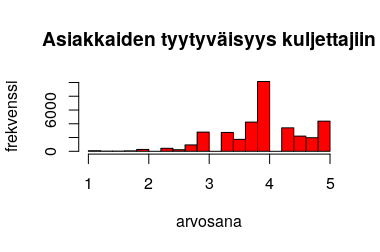
\includegraphics[width=8cm]{asty_kulj_2017_viimeinen.png}
\end{figure}
Nähdään, että jakauma on painottunut oikealle, eli vastaajat ovat enemmän tyytyväisiä kuin tyytymättömiä kuljettajiin.  
Tarkastellaan vielä yhteenveto-funktion tulostetta, joka tulostaa
frekvenssitaulun, ei-tyhjien vastausten määrän, puuttuvien vastausten määrän, keskiarvon ja varianssin edellä luetellussa järjestyksessä:  \\
\begin{lstlisting}[language=R]
[[1]]
    x.cut  Freq
1 (0.5,1]    81
2 (1,1.5]    54
3 (1.5,2]   343
4 (2,2.5]   667
5 (2.5,3]  3716
6 (3,3.5]  4478
7 (3.5,4] 14393
8 (4,4.5]  5612
9 (4.5,5]  6354

[[2]]
[1] 3.569800e+04 3.950000e+02 3.933600e+00 4.730572e-01
\end{lstlisting}
Yhteenvedon perusteella voidaan sanoa, että vastausten keskiarvo on \(\approx\) 3,9 ja keskihajonta noin 0,5. Puuttuvia vastauksia oli 395, ja ei-tyhjiä vastauksia oli 35 698. Selkeästi näkyy, että vastaajat ovat enemmän tyytyväisiä kuin tyytymättömiä kuljettajiin.
Nyt myös löytyy syy ylemmän histogrammin harvuudelle: aina kun tulee uusi tasaluku x-akselilla, niin sen perässä on tyhjä kohta. Tämä johtuu siitä että histogrammi on jaettu dataan sopimattomasti: esimerkiksi vastaajien keskiarvo "4" löytyy x-akselin kohdan "4" vasemmalta puolelta, jolloin perään tulee tyhjää tilaa. Yritetään ratkaista tämä ongelma jakamalla histogrammi isompiin palkkeihin, ja siistitään samalla kuvaajaa: \\ 
\begin{figure}[H]
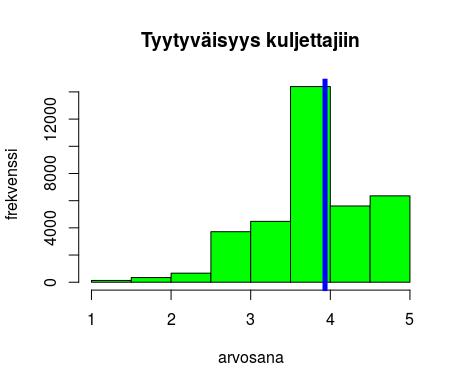
\includegraphics[width=8cm]{210517_tyytyv_kulj.png}
\end{figure}
Seuraavaksi tarkastellaan summamuuttuja -ja yhteenveto-funktioilla asiakkaiden tyytyväisyyttä erilaisiin HSL:n palveluihin. Ohessa yhteenveto-funktion tuloste:
\begin{lstlisting}[language=R]
    x.cut  Freq
1 (0.5,1]    26
2 (1,1.5]    21
3 (1.5,2]    97
4 (2,2.5]   216
5 (2.5,3]  1241
6 (3,3.5]  3159
7 (3.5,4] 10903
8 (4,4.5] 11386
9 (4.5,5]  8950

[[2]]
[1] 3.599900e+04 9.400000e+01 4.114639e+00 3.051029e-01
\end{lstlisting}
Nähdään, että yli 3/4 asiakkaista on tyytyväisiä HSL:n palveluihin (arvosana on suurempi tai yhtä suuri kuin 3,5). Nähdään myös, että keskimääräinen arvosana HSL:n palveluille oli 4,1 keskihajonnalla 0,3. Puuuttuvia vastauksia oli 94, ja ei-puuttuvia 35 999. 
\section*{2. tehtävä}
Ristiintaulukoidaan lauttasaarelaisten, tapiolalaisten ja matinkyläläisten arvosanat korvaavasta liikenteestä. Tätä varten lasketaan riviprosentit taulukosta desimaaleina: \\
\begin{lstlisting}[language=R]
               1    2    3    4    5
  Lauttasaari 0.16 0.30 0.24 0.18 0.12
  Tapiola     0.07 0.06 0.12 0.44 0.31
  Matinkyla   0.02 0.04 0.12 0.40 0.41
\end{lstlisting}
Seuraavaksi testataan väitettä H0: "postiosoitteilla ei ole yhteyttä korvaavien linjojen arvosteluun", jolloin H1 = "postiosoitteella on yhteyttä korvaavien linjojen saamaan arvosteluun",  eli onko yhteyttä asuinalueella ja muuttujalla K3A23 (korvaavan liikenteen arvostana). Tarkastellaan yhteyttä Khii neliö-testillä. Testituloksesta saamamme Khii-neliö arvo on 188.38 vapausasteilla n=8, ja p-arvo on 2,2E-16. Näin ollen jos \(\alpha\) = 0,01 niin nollahypoteesi voidaan hylätä kyseisellä merkitsevyystasolla, eli asuinalue näyttäisi vaikuttavan korvaavan liikenteen arvosanaan. \\

Seuraavaksi halutaan testata yksisuuntaisella t-testillä nollahypoteesia: \(\mu_{Lauttasaari} \geq 3\) ja sen vastaista H1-hypoteesia: \(\mu_{Lauttasaari}\) < 3. Testi tehdään merkitsevyystasolla  \(\alpha\) = 0,05.  \\
Testin perusteella nähdään, että otoskeskiarvo 2.806452 antaa vapausasteilla 216 t-arvon -2.2864, jota vastaava p-arvo on 0.0116 < 0,05. Tämän perusteella testin nollahypoteesi hylätään. Näin ollen saadusta otoksesta laskettu tulos viittisi siihen, että lauttsaarelaisten antama arvosana korvaavalle liikenteelle on pienempi kuin 3, eli voitaisiin tulkita HSL:n epäonnistuneen tavoitteissaan. \\
\section*{3. tehtävä}
Olemme kiinnostuneita selvittämään metron eri käyttäjäikäryhmien antamista arvosanoista matkustusmukavuudesta. Tätä varten laskettiin 95\% luottamusvälit metron eri käyttäjäikäryhmille, ohessa taulukko, sarakkeet x.1 ja x.2 ovat luottamusvälin päät, ja sarake x.3 on keskiarvo: \\
\begin{lstlisting}[language=R]
  Group.1      x.1      x.2      x.3
1    0-17 3.889927 4.360073 4.125000
2   18-29 3.838633 4.061367 3.950000
3   30-39 3.880753 4.079247 3.980000
4   40-65 4.059323 4.175160 4.117241
5   66-75 3.858374 4.141626 4.000000
6  75-140 3.502712 4.497288 4.000000
\end{lstlisting}
Päällepäin vaikuttaisi siltä, että eri ikäluokilla on varsin samanlaiset käsitykset matkustusmukavuudesta, joskin esimerkiksi yli 75-vuotiaiden ikäluokan luottamusväli on arvosanan mittainen (aineiston pisin), mikä on aika paljon verrattuna esimerkiksi ikäluokkaan 40-65, jossa luottamusväli on kymmenesosa-arvosanan mittainen ja aineiston lyhyin. Piirretään tilanteesta vielä kuvaaja keskiarvoista ja luottamusväleistä ikäryhmittäin:
\begin{figure}[H]
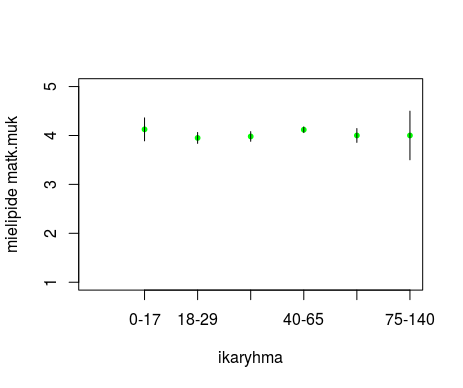
\includegraphics[width=8cm]{2305_3d.png}
\end{figure}
Nähdään, että erityisesti suurimpien ikien ikäluokalla todellakin on suurin luottamusväli vastauskeskiarvoille. Syynä vaikuttaisi olevan otoskoko, eli keski-ikäisiä vastaajia on eniten, kun taas iäkkäämpiä vastaajia vastaavasti vähiten. Voidaan vielä taulukoida ikäluokat frekvenssittäin, jolloin saadaan varmistus asiasta.
\begin{lstlisting}[language=R]
 0-17  18-29  30-39  40-65  66-75 75-140 
 1477   8162   6342  11986   1483    373 
\end{lstlisting}
Taulukosta todellakin näkyy, että suurimman ikäluokan vastaajia on erityisen vähän verrattuna muihin ikäryhmiin, ja vastaavasti 40-65-vuotiailla on erityisen suuri edustus vastaajien kesken. Tämä selittääkin hyvin luottamusvälien koot. On tietysti myös olemassa mahdollisuus, että erityisesti vanhempien ikäluokkien mielipiteissä olisi suuri hajonta, mutta tässä tapauksessa se lienee huomattavasti vähemmän merkityksellistä.
\section*{4. tehtävä}
Tehtävässä halutaan tarkastella YK-maakohtaista aineistoa, ja ensiksi työn alla on selvittää väestönkasvun ja BKT:n suhde. Tätä varten otetaan logaritmi BKT:sta, ja sovitetaan aineistolla lineaarinen malli, jossa väestönkasvu on selitettävä ja BKT(:n logaritmi) selittävä muuttuja. 
Lineaarista mallia tarkastellessa huomataan, että residuaalit ovat hyvin tasaisesti jakautuneita, mikä viittaisi siihen, että valittu malli on varsin hyvin onnistunut.
\begin{lstlisting}[language=R]
Residuals:
     Min       1Q   Median       3Q      Max 
-2.01838 -0.64747 -0.00924  0.59881  2.75867 
\end{lstlisting}
Saadun mallin yhtälö on: y= \(logBKT \cdot -0.3836 + 4.5280\), missä siis \(\beta = -0.3836\) ja vastaavasti \(\alpha = 4.5280\), missä y on väestönkasvu. Kaksisuuntaisen t-testin tulos nollahypoteesilla \(\beta = 0\) antaa p-arvoksi 1.75e-10, eli kertoimen voidaan tulkita selkeästi poikkeavan nollasta aineiston pohjalta, eli BKT:lla ja väestönkasvulla vaikuttaisi olevan jonkinlainen yhteys. \(R^2\)-selitysaste on \(\approx\) 0,27, eli BKT selittää tässä mallissa noin 27\% kaikesta vaihtelusta.
Piirretään vielä kuvaaja BKT:n logaritmin ja väestönkasvun välille, jossa eri maanosat ovat eroteltuina eri väreillä ja kaksi poikkeavaa maata annotoitu. 
\begin{figure}[H]
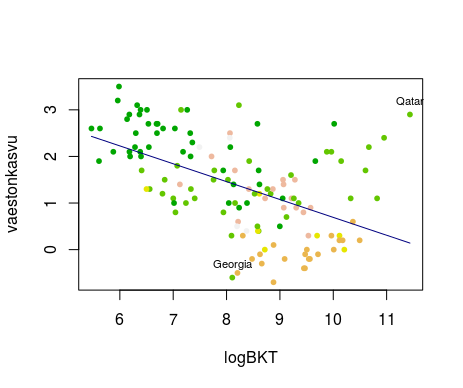
\includegraphics[width=8cm]{2305_4b.png}
\end{figure}
Seuraavaksi tarkastellaan lineaarista mallia, jossa BKT:n lisäksi toinen selittäjä on naisten lukutaito. Kun taskastellaan saatua lineaarista mallia, jossa y= \(-0.079151*logBKT -0.026272*naisten_lukutaito + 4.090062\) niin huomataan, että residuaalien 1. ja 3. kvartiili ovat symmetrisiä, ja mediaani on aika lähellä nollaa, eli mallissa vaikuttaisi olevan erityisen suuria vääristymiä. Minimiarvo ja maksimiarvo residuaaleilla ovat kyllä hieman erikokoisia, mutta niiden pohjalta ei voi vetää yhtä suuria johtopäätöksiä kuin kvartiiliarvojen perusteella.
\begin{lstlisting}[language=R]
     Min       1Q   Median       3Q      Max 
-1.51257 -0.58479 -0.05802  0.57646  2.21100 
\end{lstlisting}
Kahden selittävän muuttujan mallissa näyttäisi siltä, että t-testi antaisi hyvin pienen p-arvon (2.72e-09) naisten lukutaidolle nollahypoteesilla \(\beta_{lukutaito} = 0\), kun taas logBKT:lle varsin suuren p-arvon (0.245), eli nyt ei enää näytäkään siltä, että nollahypoteesi \(\beta_{logBKT} = 0\) ei olisikaan enää kumottavissa, kun toisena selittävänä muuttujana on naisten lukutaito! Nyt selitysarvo \(R^2\) on noin 0,4, eli jopa 40\% väestönkasvun vaihtelusta maitta voidaan selittää aineiston pohjalta BKT:lla ja naisten lukutaidolla.
Lasketaan vielä 90\% luottamusvälit saaduille kertoimille:
 \begin{lstlisting}[language=R]
                      5 %        95 %
(Intercept)          3.4129431  4.76718060
logBKT              -0.1913974  0.03309626
yk$lukutaito_naiset -0.0330724 -0.01947118
\end{lstlisting}
Nähdään, että sekä logBKT:hen että naisten lukutaitoon liittyvien kerrointen luottamusvälit ovat erisuuret, eli naisten lukutaidon tapauksessa luottamusväli on kapeampi kuin logBKT:n luottamusväli, ja logBKT:n luottamusväliin sisältyy myös nolla, joten ymmärrettävää, että nollahypoteesia:  \(\beta_{lukutaito} = 0\) testatessa t-testillä saadaan suuri p-arvo logBKT:n kertoimelle. 
Kahden selittäjän selitysaste paranee, koska naisten lukutaito on hyvä selittäjä lapsiluvulle. Erityisesti matala naisten lukutaito yhdistyy lähes poikkeuksetta kovaan väestönkasvuun. Toisaalta ilmeisesti korkea BKT ja korkea naisten lukutaito eroavat sillä tavalla toisistaan, että naisten lukutaito saattaisi selittää paremmin väestönkasvua, mitä luottamusvälien ja summary-funktion tulosteen tarkastelu antaakin olettaa?
\section*{5. tehtävä}
Ollaan saatu kolikonheitosta kuudesta heitosta neljä kruunaa, ja nyt halutaan selvittää, mikä vaikuttaisi olevan parametrin \(\theta\) (todennäköisyys saada kruuna) jakauma tällaisilla tuloksilla. Simuloidaan tapahtumaa heittämällä kolikkoa n=100 000 kertaa kuuden sarjoissa, ja valitsemalla näistä kaikki neljä heittoa saaneet sarjat. Tämän jälkeen selvitetään tämän osajoukon kolikoiden painotukset eli todennäköisyydet saada kruuna, ja näitä todennäköisyyksiä vastanneet frekvenssit. Oheisessa histogrammista näkyy simulaation tulos:
\begin{figure}[H]
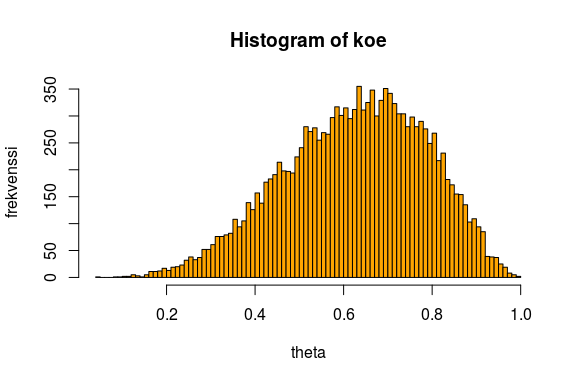
\includegraphics[width=8cm]{260517_5a.png}
\end{figure}
Nähdään, että thetan frekvenssit ovat jakautuneet siten, että eniten neljä kruunaa kuudesta ollaan saatu silloin, kun theta on ollut välillä 0,6-0,7. Ei voida myöskään sanoa, että theta on tasajakautunut, koska frekvenssit ovat eri kokoluokkaa thetan arvosta riippuen. Jakauma on oikealle vinoutunut. Kolikon painotuksen keskiarvo on \(\approx\) 0.63, ja keskihajonta \(0.1598535\). \\

Seuraavaksi simuloidaan tilannetta, jossa tiedetään, että kolikko on yksi kolikoista (1,2,3,4), joiden todennäköisyydet ovat: 1=>0,3; 2=>0,5; 3=>0,6; 4=>0,8. Oletetaan aluksi, että mahdollisuus saada tietty kolikko neljästä on diskreetisti tasajakautunut. Heitetään tämän jälkeen kolikkoa n=100 000 kertaa, ja lasketaan siitä osapopulaatiosta, jossa kuudesta heitosta saatiin neljä kruunaa, frekvenssit eri kolikoille.
\begin{figure}[H]
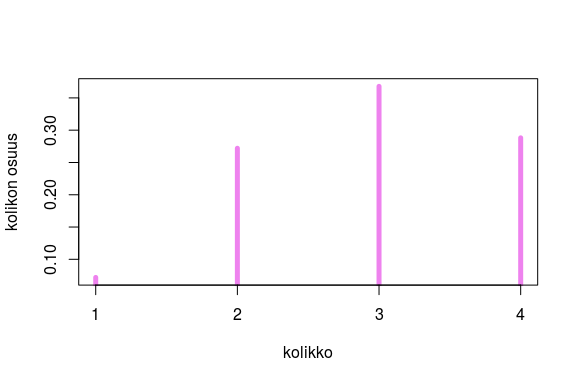
\includegraphics[width=8cm]{260517_5b.png}
\end{figure}
Histogrammista huomataan, että suurin 4/6 kruunaa saaneista heitoista osuus on kolikolla 3 (>0,3), joten todennäköisimmin Pekka heittää kolikkoa 3. Tämä vastaa myös hyvin a-kohdan simulaatiota, sillä kolikon 3 painotus on: 0,6 kruunalle.
\end{document} 





